
\documentclass[12pt]{article}
%%%\documentclass[12pt,a4paper]{scrartcl}
\usepackage[left=3cm,right=3cm,top=2cm,bottom=2cm]{geometry} % page settings
\usepackage{lingmacros}
\usepackage{tree-dvips}
\usepackage[polish]{babel}
%%% fix for \lll
\let\babellll\lll
\let\lll\relax 
\usepackage[T1]{fontenc}


\usepackage{amssymb}
\usepackage{verbatim}
\usepackage{listings}
\usepackage{amsmath}
\usepackage{amsthm}
\usepackage[boxed]{algorithm2e}
\usepackage{float}
\usepackage{graphicx}
\usepackage{csvsimple}
\usepackage{pgfplotstable}

\renewcommand{\algorithmcfname}{Algorytm}
\SetKwInput{KwData}{\textbf{Dane}}
\SetKwInput{KwResult}{\textbf{Wynik}}
\renewcommand{\qedsymbol}{$\blacksquare$}

\title{Projekt: Wycieczki}
\author{Marko Golovko}
\date{\today}

\begin{document}
\maketitle

\section*{Model konceptualny}


\subsection*{Diagram E-R}
\begin{figure}[hbt!]
 \centering
 \caption{Diagram E-R}
 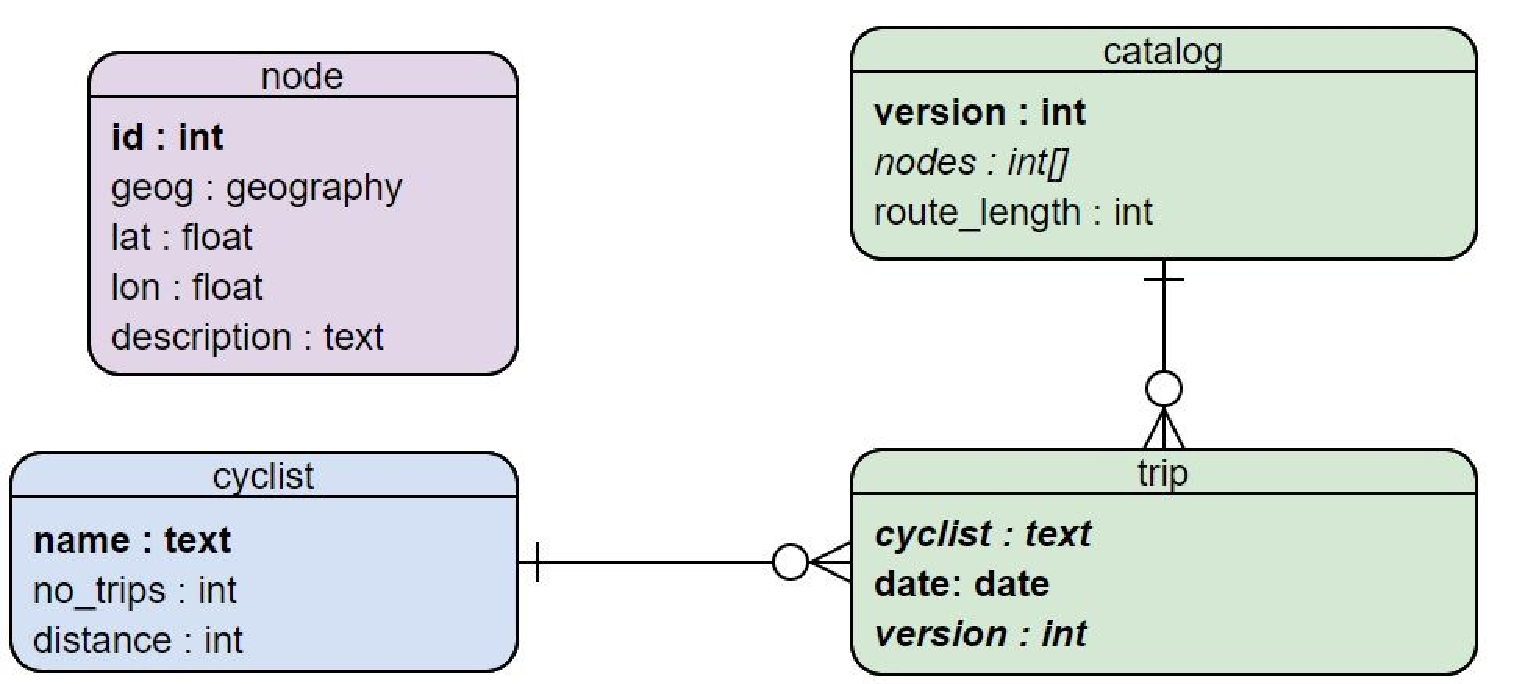
\includegraphics[width=1\textwidth]{diagram}
\end{figure}
\subsection*{Wyzwalacze}

System zawiera dwa wyzwalacze:
\begin{itemize}
  \item trip insert 
  \item catalog insert
\end{itemize}
Wyzwalacz trip insert przy dodaniu nowej wycieczki do bazy (trip) zwiększa liczbę wycieczek (no$\_$trips) i sumę metrów tych wycieczek (distance) rowerzysty (cyclist). \\
Wyzwalacz catalog insert przy dodaniu nowej trasy do bazy (catalog) na podstawie punktów (nodes) oblicza i zapisuje długość trasy (catalog.route$\_$length).
\subsection*{Funkcje API}
\begin{itemize}
  \item node dodaje nowy punkt gdzie <node> to id, za pomocą rozszerzenia PostGIS długość i szerokość geograficzną przechowuje z użyciem typu geography do geog, <lat> i <lon> odpowednio lat i lon. Wartość <description> do kolumny description tablicy node. 
  \item catalog dodaje nową trasę gdzie <version> to version, <nodes> to kolumna nodes tablicy catalog. 
  \item trip dodaje nową wycieczkę gdzie <cyclist> to cyclist, <date> to date, <version> to kolumna version tablicy trip.
  \item closest$\_$nodes znachodzi i zwraca dane punktów, z użyciem funkcji ST$\_$Distance. 
  \item party znachodzi i zwraca listę rowerzystów (różnych od <icyclist>) nocujących w promieniu 20 km od miejsca nocowania klienta <icyclist> w dniu <date>. W sposób:
  \begin{itemize}
  	\item Znachodzi punkty, w których nocują rowerzysty w dniu <date>.
  	\item Oblicza odległość punktu, w którym nocuje rowerzysta <icyclist> od punktów w których nocują rowerzysty w dniu <date>. 
  	\item Zwraca listę rowerzystów (różnych od <icyclist>) nocujących w promieniu 20 km od miejsca nocowania klienta <icyclist> w dniu <date>.
  \end{itemize}
 \item guests znachodzi rowerzystów nocujących w dniu <date>. Zwraca rowerzystów nocujących w punktu <node>.
 \item cyclist zwraca ranking rowerzystów jako wynik ograniczony do pierwszych <limit> krotek, z tablicy cyclist gdzie <no$\_$trips> to kolumna no$\_$trips i <distance> to kolumna distance.
\end{itemize}


\end{document}
